\documentclass[border=6pt]{standalone}
\usepackage{tikz}
\usetikzlibrary{arrows.meta,calc,decorations.pathreplacing}
\begin{document}
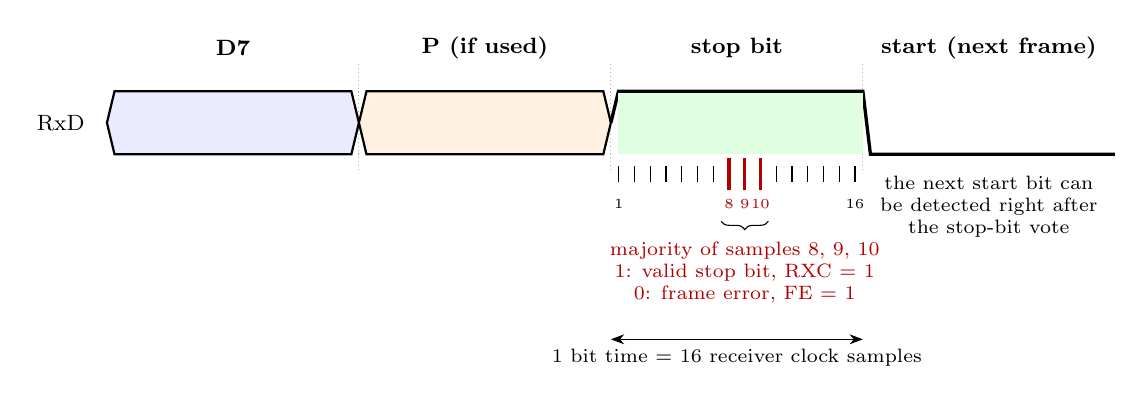
\begin{tikzpicture}[>=Stealth,font=\small,x=0.8cm,y=1cm]
% one bit time = 4 units, 16 samples per bit (normal speed)
\def\h{0.8}\def\e{0.12}
\foreach \x/\n in {2/D7,6/P (if used),10/stop bit,14/start (next frame)} \node[font=\footnotesize\bfseries] at (\x,1.35) {\n};
\foreach \x in {4,8,12} \draw[gray!60,densely dotted] (\x,-0.2) -- (\x,1.15);
\node[anchor=east,font=\footnotesize] at (-0.2,0.4) {RxD};
% D7 and P as data cells
\draw[thick,fill=blue!8] (0,0.4) -- (\e,\h) -- (4-\e,\h) -- (4,0.4) -- (4-\e,0) -- (\e,0) -- cycle;
\draw[thick,fill=orange!12] (4,0.4) -- (4+\e,\h) -- (8-\e,\h) -- (8,0.4) -- (8-\e,0) -- (4+\e,0) -- cycle;
% stop bit = 1, then the falling edge of the next start bit
\draw[very thick] (8,0.4) -- (8+\e,\h) -- (12,\h) -- (12+\e,0) -- (16,0);
\fill[green!12] (8+\e,0) rectangle (12,\h-0.02);
\draw[very thick] (8+\e,\h) -- (12,\h);
% 16 sample ticks in the stop bit
\foreach \k in {1,...,16} {
  \pgfmathsetmacro{\x}{8+(\k-0.5)*0.25}
  \draw (\x,-0.35) -- (\x,-0.15);
}
\foreach \k in {8,9,10} {
  \pgfmathsetmacro{\x}{8+(\k-0.5)*0.25}
  \draw[red!70!black,very thick] (\x,-0.45) -- (\x,-0.05);
  \node[font=\tiny,red!70!black,below] at (\x,-0.45) {\k};
}
\node[font=\tiny,below] at (8.125,-0.45) {1};
\node[font=\tiny,below] at (11.875,-0.45) {16};
\draw[decorate,decoration={brace,mirror,amplitude=3pt}] (9.75,-0.85) -- (10.5,-0.85) node[midway,below=4pt,font=\scriptsize,align=center,red!70!black]{majority of samples 8, 9, 10\\1: valid stop bit, RXC = 1\\0: frame error, FE = 1};
\draw[<->] (8,-2.35) -- (12,-2.35) node[midway,below,font=\scriptsize]{1 bit time = 16 receiver clock samples};
\node[font=\scriptsize,align=center,anchor=north] at (14,-0.15) {the next start bit can\\be detected right after\\the stop-bit vote};
\end{tikzpicture}
\end{document}
